\documentclass[polish,polish,a4paper,12pt,twoside]{article}

\usepackage[unicode]{hyperref}
\usepackage[polish]{babel}
\usepackage[T1,plmath]{polski}
\usepackage{geometry}
\usepackage[T1]{fontenc}
\usepackage[utf8]{inputenc}
\usepackage{pmboxdraw}
\usepackage{minted}
\usepackage{graphicx}
\usepackage{color}
\usepackage{pslatex}
\usepackage{anysize}
\usepackage{siunitx}
\usepackage{multicol}
\usepackage{printlen}
\usepackage{indentfirst}
\usepackage[inkscapeopt=-z, inkscapeopt=-D]{svg}
\usepackage{csquotes}
\usepackage{emptypage}

\usepackage{perpage}
\MakePerPage{footnote}

\usepackage{fancyhdr}
\fancyhf{}
\renewcommand{\headrulewidth}{0pt}
\fancyfoot[LE,RO]{\thepage}

\frenchspacing
%\usepackage{lmodern}
\selectlanguage{polish}

\usepackage[
	backend=biber,
	style=numeric,
	sorting=none
]{biblatex}
\addbibresource{thesis.bib}

\graphicspath{ {img/} }
% \setsvg{
% 	svgpath = img/
% }
% version below can't be used on linux (or more likely i couldn't make it work), leaves `/"filename.svg"` in pdf above all svg graphics. had to use the version above.
\svgpath{ {img/} }

\geometry{
	a4paper,
	left = 1.5cm,
	right = 1.5cm,
	top = 2cm,
	bottom = 2cm,
	bindingoffset = 2cm
}
\setlength{\columnsep}{-2cm}
\setlength{\baselineskip}{1.5em}
\addto\captionspolish{
	\renewcommand{\figurename}{Ryc.}
	\renewcommand{\contentsname}{Spis treści}
	\renewcommand{\listfigurename}{Indeks rycin}
	\renewcommand{\listoflistingscaption}{Indeks listingów}
}

\raggedbottom

\let\sectioncmd\section
\renewcommand{\section}{\clearpage\sectioncmd}

\title{Aplikacja mobilna na platformę Android umożliwiająca użytkowanie i uzupełnianie tworzonej społecznościowo bazy danych geoprzestrzennych}
\author{Bartosz Rodziewicz}
\date{2020}

\begin{document}
\emergencystretch 3em

\pagestyle{empty}

\begin{center}{\huge
	\noindent\textsc{Politechnika Wrocławska}\\
	\noindent\textsc{Wydział Elektroniki}\\
	\noindent\hrulefill
}\end{center}

{\large
	\noindent
	\textsc{Kierunek: Informatyka}\\*
	\textsc{Specjalność: Systemy i Sieci Komputerowe}
}

\begin{center}{\Huge
	\noindent
	\textsc{Praca Dyplomowa}\\*\medskip
	\textsc{Inżynierska}
}\end{center}

\vspace{1.75cm}

\noindent\hspace{4.6cm}\begin{minipage}[t][7.5cm][c]{10.1cm}
	\begin{center}{\large
		\noindent
		Aplikacja mobilna na platformę Android umożliwiająca użytkowanie i uzupełnianie tworzonej społecznościowo bazy danych geoprzestrzennych

		\bigskip
		\noindent
		Mobile application for the Android platform facilitating use of and contribution to a crowdsourced geospatial database

		\bigskip
		\bigskip
		\noindent
		\textsc{Autor:}\\*
		Bartosz Rodziewicz
	}\end{center}
\end{minipage}

\vspace{2cm}

\noindent\hspace{8cm}\begin{minipage}[t]{8cm}
	{\large
		\noindent
		\textsc{Prowadzący pracę:}\\*
		Dr inż. Paweł Trajdos, W4/K2

		\bigskip
		\bigskip
		\noindent
		\textsc{Ocena pracy:}\\*
	}
\end{minipage}

\vfill

\begin{center}{\large
	\noindent\hrulefill\\
	\textsc{Wrocław, 2020}
}\end{center}

\pagestyle{fancy}
\cleardoublepage

\tableofcontents
\cleardoublepage

\section{Wstęp}

W dzisiejszych czasach praktycznie każdy posiada smartfon. Większość z nich jest wyposażona w najczęściej stałe połączenie z Internetem. Pozwoliło to na wykształcenie się na rynku wielu aplikacji, których celem jest pomoc użytkownikowi w znalezieniu konkretnych informacji, w tym również geolokalizacyjnych. Istnieje wiele serwisów oferujących dostęp do map i ułatwiających znajdywanie firm (np. Google Maps\footnote{Google Maps by Google LLC — \url{https://www.google.com/maps}}, Here WeGo\footnote{Here WeGo by Here Global B.V. — \url{https://wego.here.com/}}, czy OpenStreetMaps\footnote{OpenStreetMap by OpenStreetMap Foundation — \url{https://www.openstreetmap.org/}}), wyświetlających aktualne położenie autobusów komunikacji miejskiej (np. BusLive\footnote{BusLive by BusLive Paweł Marek — \url{https://buslive.pl/}}), czy umożliwiających zlokalizowanie publicznych toalet w okolicy (np. Flush\footnote{Flush by Sam Ruston — \url{https://samruston.co.uk/}}).

Celem tej pracy jest opracowanie aplikacji na urządzenia z systemem Android umożliwiającej użytkownikom na łatwiejsze znajdywanie miejsc użyteczności publicznej, gdzie goście mają dostęp do energii elektrycznej, np. restauracji, w której można usiąść przy stoliku z laptopem i podłączyć się do prądu. Aplikacja będzie klientem do niezależnie rozwijanego serwera z bazą danych. Zaoferuje ona możliwość wyświetlania zebranych w niej danych, oraz umożliwi operowanie na nich w przystępny i szybki dla użytkownika sposób.

Program ten będzie pisany, wykorzystując zalecane przez Google metody oraz odpowiednią warstwę abstrakcji, tak aby jego dalszy rozwój był łatwy, również dla innych osób. Dodatkowo umożliwi to łatwą zmianę przechowywanych danych w bazie, jeśli w przyszłości będzie taka konieczność bądź chciano by wykorzystać ten projekt do stworzenia innej aplikacji podobnego typu.

Praca jest podzielona w następujący sposób. Rozdział \ref{concept} bardziej szczegółowo opisuje koncepcję aplikacji, jej zastosowanie i to, co zostało zrealizowane. Rozdział \ref{technology} przedstawia technologie wybrane do stworzenia programu. Rozdział \ref{implementation} opisuje aspekty implementacji kodu oraz stanowi jego dokumentację. Rozdział \ref{ui} został wykorzystany do prezentacji i opisania interfejsu użytkownika aplikacji. W rozdziale \ref{summary} zamieszone jest podsumowanie pracy. Na końcu dokumentu znajdują się odwołania do literatury, z której korzystano w trakcie przygotowywania tej pracy oraz indeks użytych rycin i listingów.

\section{Opis koncepcji}\label{concept}
	\subsection{Wymagania funkcjonalne i niefunkcjonalne}
		\subsubsection{Wymagania funkcjonalne}

			\begin{enumerate}
				\item Przeglądanie punktów w formie mapy.

					Klient oferuje możliwość przeglądania punktów w formie znaczników na mapie.

				\item Przeglądanie punktów w formie listy.

					Klient oferuje możliwość przeglądania punktów w formie listy sortowanej aktualną odległością użytkownika od punktu.

				\item Dodawanie punktów.

					Użytkownik ma możliwość dodania nowego wpisu do bazy danych.

				\item Edycja punktów.

					Użytkownik ma możliwość edycji dowolnego wpisu w bazie danych.

				\item Usuwanie punktów.

					Użytkownik ma możliwość usunięcia dowolnego wpisu w bazie danych.

				\item Przeszukiwanie bazy punktów.

					Klient oferuje możliwość ograniczenia wyświetlanych punktów na mapie do punktów spełniających określone kryteria - zawierających podany przez użytkownika ciąg znaków w polu nazwy bądź adresu.

				\item Połączenie z serwerem i synchronizacja danych.

					Aplikacja łączy się z serwerem celem synchronizacji danych. Umożliwia to użytkownikom wspólną pracę na jednej bazie danych, aktualizowanej przez każdego.

				\item Buforowanie danych z serwera na urządzeniu.

					Klient zapisuje na urządzeniu kopie bazy danych z serwera, aby umożliwić szybszy dostęp do niej oraz ograniczyć liczbę zapytań sieciowych.

				\item\label{accounts-req} System kont użytkowników.

					Aplikacja umożliwia użytkownikom założenie konta oraz zalogowanie się do niego. Dzięki temu użytkownik przestaje być anonimowy i możliwe jest zapisywanie kto dokonał jakich modyfikacji w bazie. Te informacje mogą posłużyć do zablokowania niektórym osobom możliwości edytowania danych o punktach.

				\item\label{drawing-req} System umożliwiający szkicowanie planów obiektów.

					Klient pozwala użytkownikowi dodać szkic planu budynku jako informacji o danym punkcie. Możliwe jest wgranie zdjęcia z aparatu (użytkownik robi zdjęcie planu naszkicowanego metodą tradycyjną) lub naszkicowanie cyfrowego planu w specjalnym widoku aplikacji. Widok ten ułatwia użytkownikowi szkicowanie planu poprzez możliwość układania go z gotowych kształtów poza oczywistym rysowaniem linii za pomocą palca na ekranie.

			\end{enumerate}

		\subsubsection{Wymagania niefunkcjonalne}

			\begin{enumerate}
				\item Aplikacja powinna być przygotowana na system Android.
				\item Aplikacja powinna posiadać prosty interfejs użytkownika zgodny z obowiązującymi standardami wybranej platformy.
			\end{enumerate}

	\subsection{Aplikacja mobilna}

	Pomysł na aplikację powstał podczas obserwacji innych aplikacji użytkowych, które istnieją na rynku. Głównie była ona bazowana na dwóch serwisach — aplikacji do wyszukiwania publicznych toalet (Flush\footnote{Flush by Sam Ruston — \url{https://samruston.co.uk/}}), oraz publicznych sieci Wi-Fi (WiFi Map\footnote{WiFi Map by WiFi Map LLC — \url{https://www.wifimap.io/}}). W obu przypadkach, głównym aspektem programu jest mapa ze społecznie zbieranymi danymi. Taki model działania pozwala założyć, że użytkownicy sami będą dbać o poprawność i aktualność danych.

	Tutaj też głównym miejscem jest widok mapy, umożliwiający na przeglądanie danych w łatwy dla użytkownika sposób. Dodatkowo jest możliwość wyświetlenia danych w formie listy, sortowanej rosnąco odległością od użytkownika.

	Przy uruchomieniu klient pobiera dane o wszystkich miejscach z bazy danych. Aby zmniejszyć liczbę późniejszych zapytań do serwera aplikacja zapewnia metodę na buforowanie danych na urządzeniu. Wprowadzenie takiego rozwiązania jest możliwe, ponieważ program wyświetla rzadko zmieniające się informacje. Dane przechowywane są do następnego uruchomienia, gdzie baza danych jest aktualizowana o najnowsze dane z serwera.

	Baza przechowuje podstawowe dane o miejscu, jak jego lokalizacja czy nazwa, oraz bardziej specyficzne dla tego zastosowania informacje, takie jak liczba publicznie dostępnych gniazdek, czy szkic poglądowy z zaznaczonymi punktami na planie budynku (co np. w przypadku restauracji umożliwia klientowi wybranie odpowiedniego stolika, bez konieczności pytania obsługi).

	W aplikacji jest dostępny widok szczegółowy danego miejsca, umożliwiający podejrzenie dodatkowych informacji o nim. Widok dodawania nowego miejsca umożliwia podanie wszystkich szczegółów dotyczących tego punktu, oraz miał ułatwiać dodanie planu budynku naszkicowanego ręcznie, bądź poprzez wgranie zdjęcia fizycznie wykonanego planu. Klient oczywiście pozwala również na edycje istniejących punktów, jak i usuwanie błędnie stworzonych, bądź już nieistniejących.

	\subsection{Serwer}

	Do działania aplikacja potrzebuje również internetowego serwera z bazą danych, jednak nie stanowi to przedmiotu tej pracy. Serwer jest napisany w sposób umożliwiający tej aplikacji, na połączenie się z nim, oraz wykorzystuje odpowiednią warstwę abstrakcji, by w przyszłości możliwe było stworzenie klientów na inne platformy (klient webowy, na system iOS itp.)

	\subsection{Zakres realizacji}

	W trakcie realizacji pracy wykonano większość z założonych wymagań funkcjonalnych i niefunkcjonalnych. Nie udało się jedynie zrealizować wymagań funkcjonalnych nr \ref{accounts-req} i \ref{drawing-req}, ponieważ realizacja innych wymagań zajęła więcej czasu niż było szacowane na początku pracy. Dodatkowo realizacja tych dwóch wymagań okazała się bardziej skomplikowana niż planowano. Mimo to zrealizowano całkiem solidny zakres podstawowych funkcji, który został przedstawiony na schemacie przypadków użycia na Ryc. \ref{fig:usecasediagram}. Umożliwiają one na użytkowanie programu w założonych celach oraz na jego dalszy rozwój.

	\begin{figure}[H]
		\centering
		{\scriptsize
			\includesvg[width = \textwidth]{usecasediagram}
		}
		\caption{Diagram przypadków użycia}
		\label{fig:usecasediagram}
	\end{figure}

\section{Wybrane technologie}\label{technology}
	\subsection{Platforma}

	Z punktu widzenia projektu wybór platformy mobilnej był jedynym słusznym wyborem, ponieważ aplikacja dostarcza informacje, które są potrzebne użytkownikom, gdy są w biegu, a nie siedzą w zaciszu swojego domu przed komputerem. Na rynku platform mobilnych aktualnie istnieje jedynie dwójka graczy, czyli Android od firmy Google oraz iOS od firmy Apple, mających udziały w rynku odpowiednio 77\% i 22\% \cite{mobilemarketshare}. Z tych danych wychodzi jasny obraz, że aby dotrzeć do jak największej liczby użytkowników, należy wybrać platformę Android.

	\subsection{Język programowania}

	Wybór platformy w dużej mierze uwarunkował wybór języka programowania. Istnieją oczywiście różne metody, by tworzyć oprogramowanie pod ten system, w wielu różnych językach (np. COBOL), jednak oficjalnie wspierane są następujące języki \cite{androiddevelopment}:

	\begin{itemize}
		\item Kotlin\footnote{Kotlin by Kotlin Foundation — \url{https://kotlinlang.org/}} — nowy język, działający w JVM i będący w pełni interoperacyjny z Javą, od niedawna zalecany przez Google jako główny język dla nowych aplikacji \cite{kotlinfirst};
		\item Java\footnote{Java by Oracle — \url{https://www.oracle.com/}} — standardowy język, w którym od dawna powstają aplikację na tę platformę;
		\item C++ — istnieje możliwość wykorzystania bibliotek napisanych w C++ za pomocą NDK \cite{ndk} udostępnionego przez Google, przydatne przy oprogramowaniu, dla którego kluczowa jest wydajność, czyli np. gier;
		\item HTML+CSS+JS — częściowo wspierane jest tworzenie nowoczesnych stron internetowych zachowujących się jako aplikacje wykorzystując PWA \cite{pwa}.
	\end{itemize}

	Taka sytuacja sprowadza się do wyboru pomiędzy dwoma językami: Kotlinem i Javą. Mimo pewnego wcześniejszego doświadczenia autora pracy z Javą wybrany został język Kotlin, który jest traktowany przez Google jako przyszłość dla tej platformy \cite{kotlinfirst}. Zdecydowano się na ten język, aby poznać nową technologię, która zaczyna zdobywać coraz większą popularność na rynku oraz ułatwić w przyszłości dalszy rozwój tego projektu.

	\subsection{Zewnętrzne biblioteki}

	Przy budowie projektu wykorzystano kilka zewnętrznych bibliotek, z których większość wchodzi w skład \textit{Android Framework}, czyli oficjalnych bibliotek wymaganych do tworzenia aplikacji na tę platformę.

	Podstawową użytą biblioteką jest biblioteka języka Kotlin, pozwalająca na pisanie kodu w tym języku oraz biblioteka \textit{Core} z pakietu AndroidX\footnote{Android Extension Libraries by Google and Open Handset Alliance — \url{https://developer.android.com/jetpack/androidx}}, czyli główna biblioteka wymagana przez system, implementująca podstawowe definicje takich elementów jak aktywności czy widoki programu \cite{androidapi}. Większość widoków w aplikacji stworzono wykorzystując \texttt{ConstraintLayout}, którego podstawowa definicja znajduje się w bibliotece o tej samej nazwie.

	Przy tworzeniu wykorzystano również bibliotekę \textit{AppCompat}, która pozwoliła na modyfikacje paska akcji na górze widoku aplikacji oraz implementację mechanizmu wyszukiwania miejsc.

	Do wsparcia przy budowie nawigacji pomiędzy ekranami programu wykorzystano bibliotekę o nazwie \textit{Navigation}, ponieważ jest to zalecona metoda tworzenia przejść przez Google \cite{androiddevelopment}. Z tego samego powodu wykorzystano bibliotekę \textit{Lifecycle} do lepszego wsparcia zarządzania życiem poszczególnych elementów aplikacji.

	W programie zaimplementowano bazę danych w technologii \texttt{SQLite}\footnote{SQLite by SQLite Consortium — \url{https://www.sqlite.org/}} wykorzystując bibliotekę \textit{Room}, która pozwala w prosty sposób tworzyć bazy danych do aplikacji na platformę Android.

	Do obsługi map oraz lokalizacji wykorzystano biblioteki \textit{Google Maps Services}, ponieważ jest to oficjalnie wspierana biblioteka do tych zastosowań.

	Obsługa połączenia z serwerem została zaimplementowana z pomocą biblioteki \textit{Retrofit}\footnote{Retrofit by Square — \url{https://square.github.io/retrofit}}, która pomaga w obsłudze zapytań HTTP wraz z biblioteką \textit{Moshi}\footnote{Moshi by Square — \url{https://github.com/square/moshi}}, która służy do automatyzacji parsowania danych aplikacji do \texttt{JSON} i w drugą stronę. Biblioteki \textit{Retrofit} oraz \textit{Moshi} są pierwszymi użytymi w projekcie bibliotekami niebędącymi częścią \textit{Android Framework}.

	Spoza \textit{Android Framework} wykorzystano jeszcze jedną bibliotekę — \textit{Timber}\footnote{Timber by Jake Wharton — \url{https://github.com/JakeWharton/timber}}, która znacząco ułatwia korzystanie z systemowych logów platformy Android.

	\subsection{Komunikacja z serwerem}

	Aplikacja do kontaktu z serwerem wykorzystuje jego publiczne API oparte o zapytania HTTP i architekturę typu REST \cite{restrfc}. Serwer nie posiada jeszcze domeny, więc aby się z nim połączyć konieczne jest uruchomienie go w sieci lokalnej i zmiana kodu aplikacji mobilnej podając jej poprawny adres działającego serwera. Serwer jednak nie był tematem tej pracy i został on stworzony przez inną osobę.

	Aplikacja implementuje następujące zapytania do serwera:

	\begin{itemize}
		\item pobranie wszystkich punktów z bazy danych — zapytanie typu \texttt{GET}, które zwraca listę punktów;
		\item dodanie nowego punktu — zapytanie typu \texttt{PUT}, które w ciele przyjmuje obiekt z wszystkimi parametrami miejsca (nazwa miejsca - \texttt{name}, współrzędne - \texttt{lat} i \texttt{lon}, adres - \texttt{address} oraz liczba gniazdek w lokalu - \texttt{num\_mugs}), jednak bez \texttt{Id}, zwraca dodany obiekt do bazy danych z poprawnym \texttt{Id};
		\item edycja istniejącego punktu — zapytanie typu \texttt{PATCH}, które przyjmuje zmieniony obiekt i zwraca go;
		\item usunięcie punktu — zapytanie typu \texttt{DELETE}, które przyjmuje obiekt do usunięcia i zwraca pustą odpowiedź z kodem HTTP \texttt{200}.
	\end{itemize}

	Wszystkie zapytania wykorzystują to samo URI, jednak różnią się typem i zawartością swojego ciała.

	\subsection{Środowisko deweloperskie}

	Główny telefon wykorzystany do projektu to OnePlus 5T posiadający układ Snapdragon 835 i 6GB pamięci operacyjnej działający pod kontrolą systemu Android w wersji 9 Pie z nakładką OxygenOS w wersji 9.0.9.

	Program kompilowany był z użyciem Kotlina w wersji 1.3.60 do kodu bajtowego zgodnego z JVM w wersji 1.6. Proces budowania był sterowany przez narzędzie Gradle w wersji 5.4.1 z wtyczką do Androida (\textit{Android Gradle Plugin}) w wersji 3.5.1. Kod edytowany był w środowisku deweloperskim (IDE) Android Studio w wersji 3.5.2.

	Najniższa wspierana przez aplikację wersja systemu Android to 5.0 Lollipop. Oprogramowanie było kompilowane używając SDK w wersji 29, odpowiadającej najnowszej wersji Androida — 10.

	Aplikacja została przetestowana również na następujących urządzeniach:

	\begin{itemize}
		\item OnePlus One — Android 9 Pie
		\item Xiaomi Redmi Note 5A Prime — Android 7.1.2 Nougat
		\item Nokia 8 — Android 9 Pie
		\item Samsung Galaxy Tab 8.4 Pro — Android 7.1.2 Nougat (\textit{tablet})
		\item Nexus 5X — Android 10 (\textit{maszyna wirtualna})
		\item Nexus 4 — Android 5.0 Lollipop (\textit{maszyna wirtualna})
	\end{itemize}

	Aplikacja była testowana ręcznie, a procedura testowania polegała na:

	\begin{itemize}
		\item zainstalowaniu aplikacji na urządzeniu,
		\item sprawdzeniu czy zostały pobrane wpisy z serwera,
		\item wyświetlenia tych miejsc w formie mapy i listy,
		\item przeszukaniu miejsc używając losowej nazwy punktu,
		\item dodaniu tymczasowego miejsca,
		\item edycja tego miejsca,
		\item oraz jego usunięciu.
	\end{itemize}

	Na każdym z wymienionych urządzeń aplikacja działała w pełni poprawnie. Na maszynach wirtualnych testowana była okrojona wersja aplikacji nie posiadająca funkcjonalności połączenia z serwerem z uwagi na problemy z połączeniem maszyn z serwerem znajdującym się w sieci lokalnej.

	\subsection{Kontrola wersji}

	W większości projektów informatycznych narzędzia systemu kontroli wersji pomagają zachować porządek i ułatwiają nad nim pracę \cite{git}. Z tego też powodu ten projekt również wykorzystywał narzędzie tego rodzaju — Git.

	Repozytorium Git wykorzystywane było głównie, aby lepiej zorganizować zmiany i łatwiej się w nich odnajdywać. Pozwalało na jednoczesną pracę nad kilkoma funkcjonalnościami jednocześnie, zachowując uporządkowaną historię zmian. Dodatkowo zabezpieczało ono sprawnie działający kod, pozwalając na cofnięcie niechcianych zmian w każdej chwili używając jednej komendy. System ten zapewniał też swojego rodzaju kopię zapasową, ponieważ umożliwiał on na synchronizację wszystkich zmian z serwerem serwisu GitHub, gdzie kod przechowywany był w formie prywatnego projektu.

	\subsection{System budowania}

	Do automatyzacji procesu budowania wykorzystano narzędzie Gradle\footnote{Gradle by Gradle Inc. — \url{https://gradle.org/}}. Pozwalało ono, po sprecyzowaniu podstawowych ustawień, na w pełni automatyczne tworzenie pliku \texttt{apk}, gotowego do instalacji na urządzeniu.

	W przypadku projektów na platformę Android konfiguracja Gradle podzielona jest na dwa osobne pliki — konfiguracja do całego projektu oraz poszczególnego modułu. Mimo, że projekt posiadał tylko jeden moduł, zachowany został ten podział, ponieważ uważany jest on za dobrą praktykę \cite{kotlin}.

	W pliku z globalną konfiguracją sprecyzowane zostały zdalne repozytoria, z których Gradle pobierał wymagane dependencje oraz zdefiniowane zostało użycie narzędzi wymaganych do zbudowania aplikacji na system Android.

	\begin{listing}[H]
		\caption{Konfiguracja narzędzia do budowy Gradle}
		\begin{minted}[tabsize=4,breaklines]{js}
compileSdkVersion 29
dataBinding {
	enabled = true
}
androidExtensions {
	experimental = true
}
buildToolsVersion "29.0.2"
defaultConfig {
	applicationId "test.mug.espresso"
	minSdkVersion 21
	targetSdkVersion 29
	versionCode 2
	versionName "0.1.1"
	testInstrumentationRunner "androidx.test.runner.AndroidJUnitRunner"
}
		\end{minted}
		\label{listing:gradle}
	\end{listing}

	W pliku konfiguracyjnym modułu programu znajdowały się podstawowe ustawienia, wymagane do budowy (listing \ref{listing:gradle}).

	Zdefiniowana została wersja systemu Android, użyta do budowania pliku wykonywalnego (\texttt{apk}), minimalna wersja wymagana do działania programu oraz wersja narzędzia używanego do budowania. Aktywowano technologię data binding, która w prosty sposób umożliwia tworzenie powiązań pomiędzy kodem a definicją układu widoku oraz aktywowano eksperymentalne funkcjonalności \texttt{Android Framework}.

	Ustalona została nazwa kodowa programu oraz jego wersja. Zgodnie z konwencją systemu Android zalecane jest użycie jako nazwy kodowej odwrotności domeny przeznaczonej dla danej aplikacji. Z uwagi, że do projektu nie została zarejestrowana jeszcze żadna domena, na czas realizacji pracy zdecydowano się użyć domeny \texttt{test}, która przeznaczona jest do użycia w testowaniu oprogramowania i gwarantuje pewność, że nigdy nie nastąpi konflikt z żadną istniejącą domeną, ponieważ zablokowana jest możliwość jej rejestracji \cite{testdomainrfc}.

	\subsection{Testy jednostkowe}

	Do projektu podłączono biblioteki \textit{JUnit} umożliwiające pisanie lokalnych testów jednostkowych oraz testów wykonywanych na fizycznym urządzeniu. Niestety z uwagi na ograniczenia czasowe do aplikacji nie powstały żadne testy.

\section{Opis implementacji}\label{implementation}
	\subsection{Struktura}
		\subsubsection{Podział plików w projekcie}

		Nawet prosty projekt na platformę Android ma dość skomplikowaną strukturę plików i wymaga chwili na zapoznanie się z nią.

		Aplikacje na ten system pisane są w formie modułowej. Ten projekt posiada tylko jeden moduł, który nazywa się \texttt{app}.

		W głównym folderze projektu znajduje się kilka plików konfiguracyjnych dla narzędzia \textit{Gradle}, które służy do automatyzacji procesu budowania. Folder \texttt{.idea/} zawiera pliki konfiguracyjne środowiska IDE — Android Studio.

		Wszystkie pliki w folderze \texttt{app/} to pliki należące do tego modułu, folder \texttt{app/src/} zawiera 5 podfolderów, które wprowadzają podstawowy podział kodu aplikacji:

		\begin{itemize}
			\item \texttt{main/} zawiera kod wspólny dla wszystkich metod budowania,
			\item \texttt{debug/} to kod przeznaczony do budowania w tym trybie,
			\item \texttt{release/} to kod przeznaczony do użycia przy budowaniu w trybie release, w tym projekcie te dwa powyższe foldery są używane do przechowywania osobnych plików z kluczem \texttt{API} do Google Maps,
			\item \texttt{test/} i \texttt{androidTest/} to foldery wykorzystywane przez testy jednostkowe.
		\end{itemize}

		Główny podział kodu znajduje się w katalogu \texttt{app/src/main/}:

		\begin{itemize}
			\item folder \texttt{java/} zawiera kod pisany w języku Java lub Kotlin (w tym projekcie tylko Kotlin), struktura pod folderów odpowiada nazwie kodowej aplikacji,
			\item folder \texttt{res/} zawierający zasoby zapisane w formacie \texttt{XML}, gdzie najważniejsze to pliki definicji układu widoków (\texttt{res/layout/}) oraz definicji menu (\texttt{res/menu/}),
			\item \texttt{AndroidManifest.xml} — plik informujący system Android o strukturze tej aplikacji.
		\end{itemize}

		\subsubsection{Przepływ danych}

		\begin{figure}[H]
			\centering
			\includesvg[width = \textwidth]{architecture}
			\caption{Schemat architektury}
			\label{fig:architecture}
		\end{figure}

		Z perspektywy obsługi danych architektura aplikacji była pisana wzorując się na sugerowanej przez Google strukturze \cite{googlearch}\cite{kotlin}. Została ona przedstawiona na Ryc. \ref{fig:architecture}. Polega ona na tym, że klasa reprezentująca Aktywność bądź Fragment posiada członka będącego ViewModelem, ViewModel zawiera członka klasy Repozytorium, a Repozytorium członków klas Bazy Danych i klasy do obsługi połączeń sieciowych. Relacja zawierania jest na schemacie przedstawiona ciągłą linią. Aby jednak w takim układzie ViewModel mógł wpływać na kod w Aktyności/Fragmencie wykorzystywane są zmienne typu LiveData z ustawionymi obserwatorami w klasie Aktywności/Fragmentu. Zmiana wartości zmiennej powoduje poinformowanie obserwatorów i wykonanie kodu obserwatora. Ten rodzaj niebezpośredniego oddziaływania jest na schemacie przedstawiony linią przerywaną.

		Stworzona została klasa pełniąca funkcję repozytorium, które jest pośrednikiem w dostępie do danych z bazy oraz obsługuje zapytania sieciowe, by aktualizować dane znajdujące się w niej. Dostęp do repozytorium wykonywany jest z poziomu klas typu \texttt{ViewModel}. Starano się w nich zawrzeć jak największą część kodu odpowiedzialnego za manipulowanie danymi. W klasach aktywności i fragmentów starano się zostawić tylko kod odpowiedzialny za obsługę interfejsu użytkownika. Odświeżanie danych wyświetlanych na ekranie wykonywane jest z poziomu klas \texttt{ViewModel} korzystając ze zmiennych typu \texttt{LiveData} i technologii data binding.

		\begin{listing}[H]
			\caption{Lista plików z kodem źródłowym (\textit{Pliki są wyświetlone w ręcznie ustalonej kolejności})}
			\begin{minted}[tabsize=4,breaklines]{text}
├── EspressoApplication.kt
├── mainView
│   ├── DataViewModel.kt
│   ├── ListViewFragment.kt
│   ├── MainActivity.kt
│   └── MapViewFragment.kt
├── detailView
│   ├── DetailViewFragment.kt
│   └── DetailViewModel.kt
├── addEditView
│   ├── AddViewFragment.kt
│   └── AddViewModel.kt
├── domain
│   ├── PowerMug.kt
│   └── PowerMugWithDistance.kt
├── repository
│   └── PowerMugRepository.kt
├── database
│   ├── DbPowerMug.kt
│   ├── PowerMugDatabase.kt
│   └── PowerMugDatabaseDao.kt
├── network
│   ├── NetworkPowerMug.kt
│   └── ServerApiService.kt
├── BindingAdapters.kt
└── Utils.kt
			\end{minted}
			\label{listing:files}
		\end{listing}

		Schemat ten ma swoje odbicie w układzie plików z folderu zawierającego kod źródłowy (listing \ref{listing:files}).

		Aplikacja składa się z jednej aktywności, której jedynym zadaniem jest załadowanie odpowiedniego pełnoekranowego fragmentu.

		Do każdego fragmentu (widoku) stworzony został odpowiedni ViewModel, z wyjątkiem dwóch głównych fragmentów — \texttt{MapView} i \texttt{ListView}, które posiadają jeden wspólny obiekt tego typu.

		Klasy reprezentujące struktury używane przez ViewModel zostały wydzielone do folderu \texttt{domain}. W kolejnych folderach pogrupowane są klasy wykorzystywane przez repozytorium, bazę danych i obsługę sieci.

		Na samym końcu znajdują się dwa zbiorcze pliki zawierające pomocnicze wolne funkcje (niebędące częścią żadnej klasy).


		\subsubsection{Widoki i nawigacja}

		\begin{figure}[H]
			\centering
			{\scriptsize
				\includesvg[width = 0.5\textwidth]{navigation}
			}
			\caption{Diagram nawigacji pomiędzy fragmentami}
			\label{fig:navigation}
		\end{figure}

		Aplikacja posiada jedną aktywność i cztery widoki, w tym dwa główne. Aktywność przy tworzeniu aktywuje szablon nawigacji (znajdujący się w \texttt{res/navigation/}), który pomaga w bezproblemowym zarządzaniu przechodzeniem pomiędzy fragmentami. Schematyczny diagram tego szablonu został przedstawiony na Ryc. \ref{fig:navigation}. Przedstawia on wszystkie fragmenty stworzone w aplikacji i możliwe przejścia pomiędzy nimi. Dokładny opis tych widoków z punktu widzenia użytkownika znajduje się w rozdziale \ref{ui}. Ten rozdział opisuje je z perspektywy nawigacji w aplikacji i przejść pomiędzy nimi.

		Głównym i domyślnym widokiem jest widok mapy. Jego wygląd dla użytkownika znajduje się na lewej połowie Ryc. \ref{fig:screenshotmain}. Uruchamia się on zaraz po starcie aplikacji. Umożliwia przeglądanie danych w postaci punktów na mapie zajmującej cały ekran. Kliknięcie w punkt powoduje wyświetlenie szczegółów danego miejsca.

		Drugim głównym widokiem jest widok pozwalający na wyświetlenie miejsc w formie sortowanej listy. Jego wygląd znajduje się na prawej połowie Ryc. \ref{fig:screenshotmain}. Przejście do niego jest możliwe z ekranu mapy za pomocą przycisku na dole. Kliknięcie pozycji reprezentującej konkretne miejsce powoduje wyświetlenie się jego szczegółów. Ten widok znajduje się na Ryc. \ref{fig:screenshotdetail}.

		Oba widoki główne posiadają przycisk do dodania nowego miejsca, który przenosi do widoku dodawania. Ten widok znajduje się na Ryc. \ref{fig:screenshotaddedit}. Po dodaniu następuje przejście do ekranu mapy. Ekran ze szczegółami poza wyświetlaniem dodatkowych informacji o miejscu pozwala na usunięcie miejsca z bazy. Po usunięciu następuje przejście do widoku mapy.

		Android oferuje dwa rodzaje przejść pomiędzy ekranami \cite{androiddevelopment} — te opisane wyżej to przejścia w przód, które wykonywane są poprzez interakcje użytkownika z aplikacją. Drugim typem przejść są przejścia w tył wykonywane przez użycie przycisku wstecz. Tego typu przejścia powracają do poprzedniego ekranu. Aby nawigacja w aplikacji działała poprawnie i intuicyjnie dla użytkownika wszystkie przejścia "w przód" powracające do ekranu mapy powodują wyczyszczenie kolejki wcześniejszych widoków, aby kliknięcie przycisku wstecz na widoku mapy powodowało opuszczenie aplikacji.

	\subsection{Uruchomienie aplikacji i załadowanie mapy}

	Pierwszym krokiem po uruchomieniu aplikacji jest wykonanie się kodu z klasy Aplikacji (\texttt{EspressoApplication.kt}). Kod tam znajdujący się należy ograniczyć do minimum \cite{kotlin} i w tym projekcie znajduje się tam jedynie aktywacja zewnętrznej biblioteki \textit{Timber} pomagającej w tworzeniu logów.

	Następnie tworzona jest aktywność, która aktywuje szablon nawigacji ładujący główny widok, którym jest ekran mapy.

	Podczas tworzenia się widoku mapy (metoda \texttt{onCreateView()}) następuje załadowanie definicji układu elementów widoku (znajdującej się w \texttt{res/layout/}). Dzięki wykorzystaniu data binding już w pliku \texttt{layout} przypisane są odpowiednie metody z ViewModela, które mają się wykonać po kliknięciu przycisków. Następnie jest tworzona (bądź podłączona, jeśli już istnieje) instancja klasy \texttt{ViewModel} dla tego widoku.

	Przy tworzeniu ViewModel, tworzona jest instancja repozytorium. Po stworzeniu repozytorium zostaje momentalnie zwrócona lista miejsc znajdująca się w bazie i następuje żądanie aktualizacji bazy poprzez połączenie z serwerem. Takie działanie powoduje, że użytkownik od razu po uruchomieniu aplikacji może z niej korzystać, zamiast czekać na pobranie się danych z serwera, które wcale nie musiały ulec zmianie. Po zakończeniu procesu pobierania repozytorium aktualizuje w tle dane w bazie oraz dzięki data binding zmiany te propagują się do wszystkich widoków aplikacji.

	Po stworzeniu ViewModela następuje stworzenie obserwatorów zmiennych \texttt{LiveData} w ViewModelu używanych do nawigacji oraz żądanie inicjalizacji mapy do biblioteki \texttt{Google Maps Services} i zapytanie użytkownika o pozwolenie na dostęp do lokalizacji (jeśli wcześniej nie zostało ono udzielone).

	Po poprawnej inicjalizacji mapy następuje stworzenie obserwatora listy punktów i wypełnienie mapy punktami. Następuje też przypisanie działania, które ma się wykonać po kliknięciu na dany punkt. Widok mapy przechodzi na aktualną pozycję użytkownika.

	Obecność elementu mapy zaburza poprawną implementację wzorca projektowego MVVM (Model-View-ViewModel) \cite{mvvmarticle}, ponieważ zgodnie z nim część kodu odpowiedzialnego za obsługę map powinna zostać przeniesiona do ViewModela. Nie udało się tego jednak dokonać podczas realizacji tego projektu, z uwagi na poziom skomplikowania kodu wymaganego do obsługi tego elementu.

	\subsection{Wyszukiwanie punktów}

	Aplikacja oferuje wyszukiwanie punktów po nazwie lub adresie. Przeszukiwanie dostępne jest z poziomu przycisku znajdującego się na panelu na górze ekranu mapy.

	Przy tworzeniu menu (w trakcie tworzenia widoku) do obiektu wyszukiwania przypisywany jest \texttt{queryTextListener}, który zawiera definicje metody, którą należy wywołać po zatwierdzeniu wyszukiwania.

	Wyszukiwanie polega na wykonaniu \texttt{queryTextListener.onQueryTextSubmit(String)} \cite{androidapi}, czyli wysłaniu do repozytorium tekstu z pola wyszukiwania i czekaniu na wyniki. Repozytorium odpytuje bazę danych i zwraca do ViewModelu listę znalezionych miejsc.

	Po pojawieniu się wyników mapa jest czyszczona i pokazywane są na niej tylko znalezione miejsca, oraz widok automatycznie przechodzi na pierwszy znaleziony punkt. W przypadku braku wyników pojawia się stosowny komunikat.

	Powrót do wyświetlania wszystkich miejsc jest możliwy poprzez wyjście z wyszukiwania przyciskiem na górnym pasku aplikacji. Następuje wtedy wywołanie metody \texttt{closeListener}, która czyści mapę i ponownie ustawia obserwatora na domyślną zmienną \texttt{LiveData} z listą wszystkich miejsc.

	\subsection{Przejście z użyciem data binding}\label{navigation}

	Większość przejść w tym projekcie realizowana jest zgodnie z poniższym schematem. Jest to zalecana metoda wykonywania przejść, ponieważ już w definicji układu widoku widać, do czego służy dany przycisk \cite{kotlin}.

	\begin{listing}[H]
		\caption{Kod znajdujący się w klasie typu ViewModel potrzebny do przejścia}
		\begin{minted}[tabsize=4,breaklines]{java}
private var _navigateToSecondView = MutableLiveData<Boolean>()
val navigateToSecondView: LiveData<Boolean>
	get() = _navigateToSecondView

fun goToSecondView() {
	_navigateToSecondView.value = true
}

fun wentToSecondView() {
	_navigateToSecondView.value = false
}
		\end{minted}
		\label{listing:navigationviewmodel}
	\end{listing}

	\begin{listing}[H]
		\caption{Kod obserwatora potrzebny do przejścia}
		\begin{minted}[tabsize=4,breaklines]{java}
viewModel.navigateToSecondView.observe(viewLifecycleOwner, Observer {
		if (it == true) {
			this.findNavController()
				.navigate(R.id.action_mapViewFragment_to_listViewFragment)
			viewModel.wentToSecondView()
		}
	})
		\end{minted}
		\label{listing:navigationview}
	\end{listing}

	Metoda polega na przypisaniu na kliknięcie w definicji układu widoku metody z ViewModela (w tym wypadku \texttt{goToSecondView()}). Metoda ta, zmienia wartość zmiennej \texttt{LiveData} (listing \ref{listing:navigationviewmodel}) na którą ustawiony jest obserwator w widoku (listing \ref{listing:navigationview}), który aktywuje się jeśli zmienna ma wartość \texttt{true}. Wywołuje on kontroler nawigacji i wykonuje odpowiednie przejście, po czym ustawia zmienną \texttt{LiveData} (w tym wypadku \texttt{\_navigateToSecondView}) na \texttt{false} wykorzystując drugą metodę (w tym wypadku \texttt{wentToSecondView()}). Ustawienie jej bezpośrednio jest niemożliwe, ponieważ jest to zmienna prywatna, a \texttt{navigateToSecondView} jest zmienną publiczną, której wartość nie może być modyfikowana — jest to zdefiniowane w ten sposób, aby zachować enkapsulację klasy.

	Konieczność wykonania takiego przepływu jest spowodowana faktem, że użycie kontrolera nawigacji jest możliwe tylko z poziomu kodu fragmentu, a nie kodu ViewModela \cite{androidapi}.

	\subsection{Wyświetlenie listy miejsc}

	Wyświetlenie listy miejsc wymaga przejścia do widoku listy. Przejście z widoku mapy do widoku listy jest użyte jako przykład do opisu przejścia w podrozdziale powyżej.

	Zaimplementowany w tym projekcie widok listy wykorzystuje specjalny widok \texttt{Android Framework} o nazwie \texttt{RecyclerView}. Jest to widok przystosowany do wyświetlania bardzo dużych zbiorów danych bez wpływu na pamięć urządzenia. Widok ten, zamiast tworzyć jedną długą listę i wyświetlać tylko jej fragment, tworzy listę zawierająco niewiele więcej elementów niż mieści się w danej chwili na ekranie i wraz z jej przewijaniem ponownie wykorzystuje obiekty w pamięci, które znikają z ekranu, aby wyświetlić nowe obiekty. Do działania wymaga definicji dodatkowego obiektu typu \texttt{ViewAdapter} \cite{androidapi}.

	Do stworzenia obiektu \texttt{ViewAdapter} wymagany jest obiekt \texttt{ViewHolder}, który operuje na definicji układu widoku pojedynczego elementu z listy. W tak podstawowej liście jak w tym projekcie obiekt ten nie definiuje nic poza nazwą używanej definicji układu.

	Nawigacja do tego fragmentu powołuje wywołanie metody \texttt{onCreateView()}, która na samym początku ładuje definicję układu widoku oraz przypisuje się do ViewModela (tego samego co \texttt{mapView}, więc przechodząc z niego mamy pewność, że ten ViewModel już istnieje).

	Z uwagi na brak konieczności ładowania mapy już na tym etapie ustawiani są obserwatorzy na zmienne wykorzystywane do nawigacji, jak i zmienne z listą punktów. Ten widok z uwagi na konieczność sortowania listy po odległości wykorzystuje jednak inną listę niż widok mapy. Lista potrzebna do tego widoku jest zdefiniowana w ViewModelu i jest tworzona w formie transformacji podstawowej listy wykorzystując dodatkowo aktualną lokalizację użytkownika.

	Do obliczenia odległości pomiędzy lokalizacją użytkownika a punktem wykorzystywany jest wzór \ref{eq:1}, który zabezpiecza przed błędami zaokrągleń wynikających z precyzji arytmetyki zmiennoprzecinkowej \cite{haversineformulaarticle}.

	\begin{equation}
d = 2r\arcsin(\sqrt{\sin^2(\frac{\varphi_1-\varphi_2}{2})+\cos(\varphi_1)\cos(\varphi_2)\sin^2(\frac{\lambda_1-\lambda_2}{2})}),\label{eq:1}
	\end{equation}
	gdzie:
	\begin{itemize}
		\item $ d $: odległość, pomiędzy dwoma punktami [w kilometrach];
		\item $ \varphi_1, \varphi_2 $: szerokość geograficzna punktu 1 i punktu 2 [w radianach];
		\item $ \lambda_1, \lambda_2 $: wysokość geograficzna punktu 1 i punktu 2 [w radianach];
		\item $ r $: uśredniony promień kuli ziemnskiej [w kilomentrach].
	\end{itemize}

	Na samym końcu tworzony jest obiekt typu \texttt{ViewAdapter} i zostaje on przypisany do parametrów \texttt{RecyclerView}.

	\subsection{Wyświetlenie widoku szczegółów}

	Przejście do tego fragmentu jest możliwe po kliknięciu w znacznik na mapie w widoku mapy bądź pozycje na liście w widoku listy. Przy przejściu następuje przekazanie jednego parametru (\texttt{Id} obiektu), którego szczegóły mają zostać wyświetlone.

	Tworzenie widoku rozpoczyna od załadowania definicji układu widoku i uzyskanie dostępu do repozytorium. Następnie wykonywane jest zapytanie do repozytorium o obiekt podając jego \texttt{Id}. Zapytanie nie korzysta z bazy danych, więc wykonywane jest na głównym wątku. Po otrzymaniu obiektu tworzony jest ViewModel wykorzystując do tego wzorzec projektowy fabryki (stworzenie ViewModela z parametrami w konstruktorze wymaga zdefiniowania dodatkowej klasy, pełniącej rolę fabryki).

	Następnie tworzeni są obserwatorzy zmiennych używanych do nawigacji, następuje żądanie inicjalizacji mapy oraz uzupełnione zostaje menu w pasku na górze ekranu.

	Po inicjalizacji mapy kamera zostaje przeniesiona na marker miejsca.

	\subsection{Usuwanie obiektu}

	Usunięcie wybranego obiektu jest możliwe poprzez opcję w menu na pasku akcji. Schemat wykorzystany do usuwania jest podobny do schematu przejścia opisanego w rozdziale \ref{navigation}.

	W momencie wybrania opcji następuje wyświetlenie nieskończonego paska postępu oraz zapytanie do repozytorium o usunięcie obiektu. Z uwagi na wykonywanie zapytania do serwera oraz do lokalnej bazy działanie to musi być wykonane na osobnym wątku.

	Po obsłużeniu zapytania repozytorium zwraca \texttt{Boolean}, czy udało się usuwanie, czy nie. Bazując na nim ustawiana jest trzystanowa LiveData, której obserwator podejmuje stosowne działanie przy zmianie wartości.

	Gdy usuwanie się uda następuje przejście do widoku mapy, w razie niepowodzenia pokazany zostaje komunikat i znika pasek postępu. Po obsłużeniu tej zmiany UI zmienna jest przywracana do stanu \texttt{UNSET}.

	\subsection{Dodawanie/edycja obiektu}

	Aby wykonać dodanie bądź edycję obiektu konieczne jest przejście do fragmentu \texttt{addViewFragment}. Dodanie jest możliwe z obu głównych widoków, natomiast edycja z widoku szczegółów. Wywołanie nawigacji wymaga podania \texttt{Id} zmienianego miejsca. Jeśli przejście następuje w celu stworzenia nowego obiektu, podawany jest parametr \texttt{-1}. Jest to specjalnie zarezerwowany \texttt{Id}, który nigdy nie może pojawić się jako poprawny \texttt{Id} w bazie danych.

	Stworzenie widoku wygląda bardzo podobnie do widoku szczegółów. Jeśli podanym argumentem jest \texttt{-1}, zamiast poprawnego obiektu, do ViewModela przekazywany jest \texttt{null}. Następuje żądanie inicjalizacji map i dostępu do lokalizacji użytkownika. Następnie tworzony jest pusty obiekt w ViewModelu i uzupełniany aktualną lokalizacją użytkownika. Na mapie w tym miejscu pojawia się też marker.

	Jeśli został podany \texttt{Id} poprawnego miejsca ViewModel, jest tworzony z tym obiektem i po inicjalizacji map kamera przechodzi do lokalizacji edytowanego miejsca, a pola do edycji parametrów miejsca uzupełniają się aktualnymi wartościami.

	Kliknięcie na jakiekolwiek miejsce na mapie powoduje przeniesienie wskaźnika w nowe miejsca.

	Zapisanie dodania/edycji miejsca możliwe jest poprzez użycie przycisku na dole ekranu. Wykorzystywany jest podobny schemat jak przy usuwaniu i przejściu. Wysyłane jest wtedy odpowiednie zapytanie do repozytorium i następuje oczekiwanie na wynik. Przy poprawnej akcji program przechodzi do widoku mapy, przy negatywnym następuje informacja o błędzie.

	\subsection{Implementacja repozytorium}

	Model repozytorium w tym projekcie pełni funkcję warstwy abstrakcji pomiędzy zapytaniami do serwera i bazy oraz powoduje skupienie całego kodu odpowiedzialnego za te operacje w jednym miejscu. Repozytorium jest zaimplementowane w formie wzorca projektowego typu Singleton, zapewniającego, że w trakcie życia aplikacji będzie istniał tylko jeden obiekt repozytorium i bazy danych \cite{designpatterns}.

	\begin{listing}[H]
		\caption{Publiczny interfejs repozytorium}
		\begin{minted}[tabsize=4,breaklines]{java}
val powerMugs: LiveData<List<PowerMug>>

suspend fun refreshCache()

suspend fun updatePlace(powerMug: PowerMug): Boolean
suspend fun insertPlace(powerMug: PowerMug): Boolean
suspend fun deletePlace(powerMug: PowerMug): Boolean

fun search(query: String): LiveData<List<PowerMug>>

fun returnPlace(key: Long): PowerMug?
		\end{minted}
		\label{listing:repository}
	\end{listing}

	Użycie repozytorium sprowadza się do wywołania jednej z publicznych metod jego interfejsu z dowolnego miejsca aplikacji. Metody wypisane są w listingu \ref{listing:repository}.

	Użycie metod typu \texttt{suspend} konieczne jest z poziomu współprogramów (\textit{ang.} coroutines) \cite{kotlindocs}, aby zapobiec blokowaniu wątku głównego programu odpowiedzialnego za wyświetlanie elementów interfejsu użytkownika.

	Wszystkie metody działające we współprogramach mają podobny schemat działania — najpierw konkretne działanie jest wykonywane na serwerze, po czym w przypadku powodzenia zmiana zapisywana jest w lokalnej bazie danych, z której korzysta program. Zwracany obiekt typu \texttt{Boolean} informuje o sukcesie bądź niepowodzeniu danej akcji.

	\subsection{Przechowywanie obiektów}

	Mimo, że program w każdym miejscu wykorzystuje bardzo podobną definicję klasy poszczególnego punktu na mapie, zdecydowano się rozdzielić ich definicje na 3 osobne — definicję dla logiki programu (domenową — \texttt{PowerMug}), do bazy danych (\texttt{DbPowerMug}) i do zapytań sieciowych (\texttt{NetworkPowerMug} oraz \texttt{EphemeralNetworkPowerMug}). Tego typu rozdzielenie nie było konieczne, jednak powoduje, że kod aplikacji staje się bardziej elastyczny i modyfikacja np. modelu bazy nie powoduje konieczności wprowadzenia modyfikacji w kodzie całej aplikacji.

	\begin{listing}[H]
		\caption{Metody używane do konwersji pomiędzy modelami obiektów}
		\begin{minted}[tabsize=4,breaklines]{java}
fun PowerMug.asDbModel(): DbPowerMug
fun PowerMug.asNetworkModel(): NetworkPowerMug
fun PowerMug.asEphemeralNetworkModel(): EphemeralNetworkPowerMug

fun DbPowerMug.asDomainModel(): PowerMug
fun List<DbPowerMug>.asDomainModel(): List<PowerMug>

fun NetworkPowerMug.asDatabaseModel(): DbPowerMug
fun List<NetworkPowerMug>.asDatabaseModel(): Array<DbPowerMug>
		\end{minted}
		\label{listing:modelconversion}
	\end{listing}

	Aby uprościć zamianę obiektów, jednej reprezentacji w drugą przygotowano specjalne metody poszczególnych klas (listing \ref{listing:modelconversion}).

\section{Opis interfejsu użytkownika}\label{ui}

Program posiada zaimplementowany interfejs użytkownika w dwóch językach — angielskim i polskim. W tej pracy wszystkie zdjęcia ukazują interfejs polski, aby zachować zgodność językową z językiem dokumentu.

	\subsection{Ekrany główne}

	\begin{figure}[H]
		\centering
		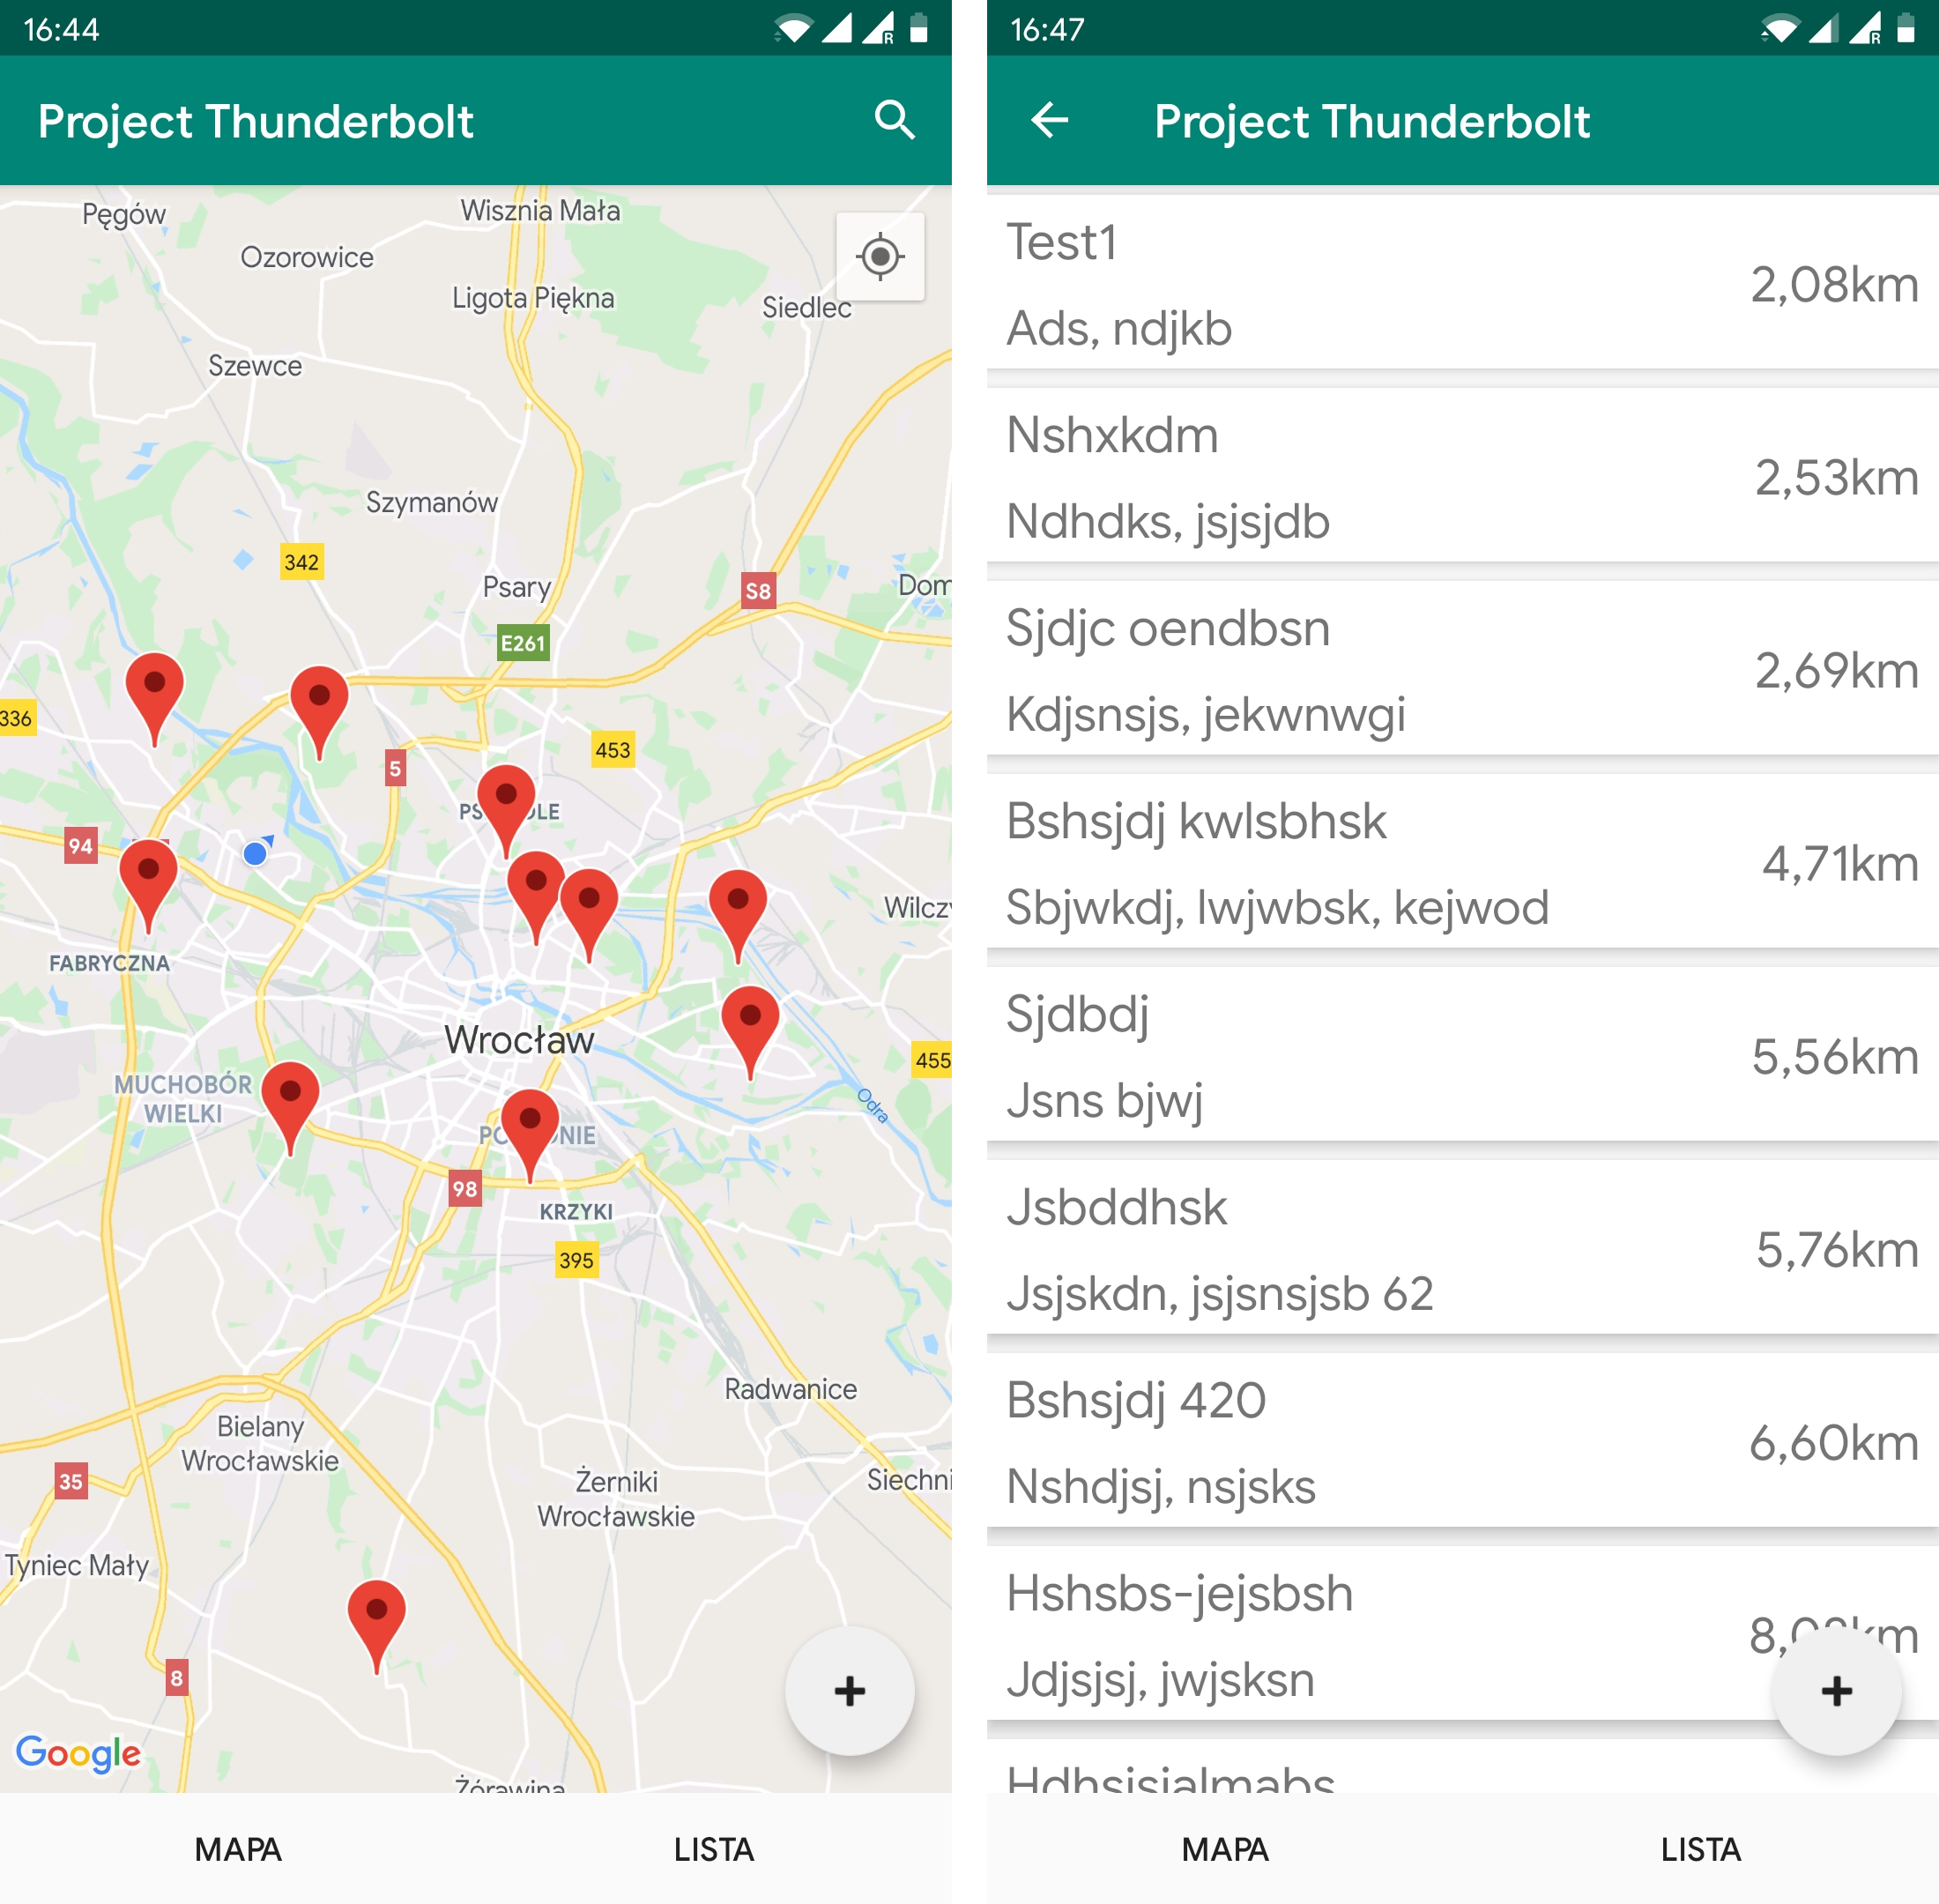
\includegraphics[width = 0.7\textwidth]{screenshot-main}
		\caption{Dwa główne widoki programu}
		\label{fig:screenshotmain}
	\end{figure}

	Aplikacja posiada dwa główne ekrany — widok mapy i widok listy. Ich wygląd został przedstawiony na Ryc. \ref{fig:screenshotmain}. Oba posiadają pasek na dole służący do nawigacji i przełączania pomiędzy nimi. W prawym dolnym rogu każdego z nich znajduje się "pływający" przycisk służący do dodawania nowego obiektu.

	Na widoku mapy cały ekran zajęty jest przez fragment Google Maps, wyświetlający wszystkie punkty w formie markerów w odpowiednich miejscach geograficznych. Kliknięcie danego markera przenosi do ekranu ze szczegółami o konkretnym miejscu. Na górnym pasku poza nazwą aplikacji wyświetlany jest przycisk uruchamiający tryb wyszukiwania.

	W formie listy cały ekran jest zajęty przez przewijaną listę miejsc, posortowaną rosnąco odległością od aktualnej lokalizacji użytkownika. Kliknięcie w dowolną pozycję na liście powoduje przeniesienie do ekranu ze szczegółami o tym miejscu.

	\subsection{Wyszukiwanie punktów}

	\begin{figure}[H]
		\centering
		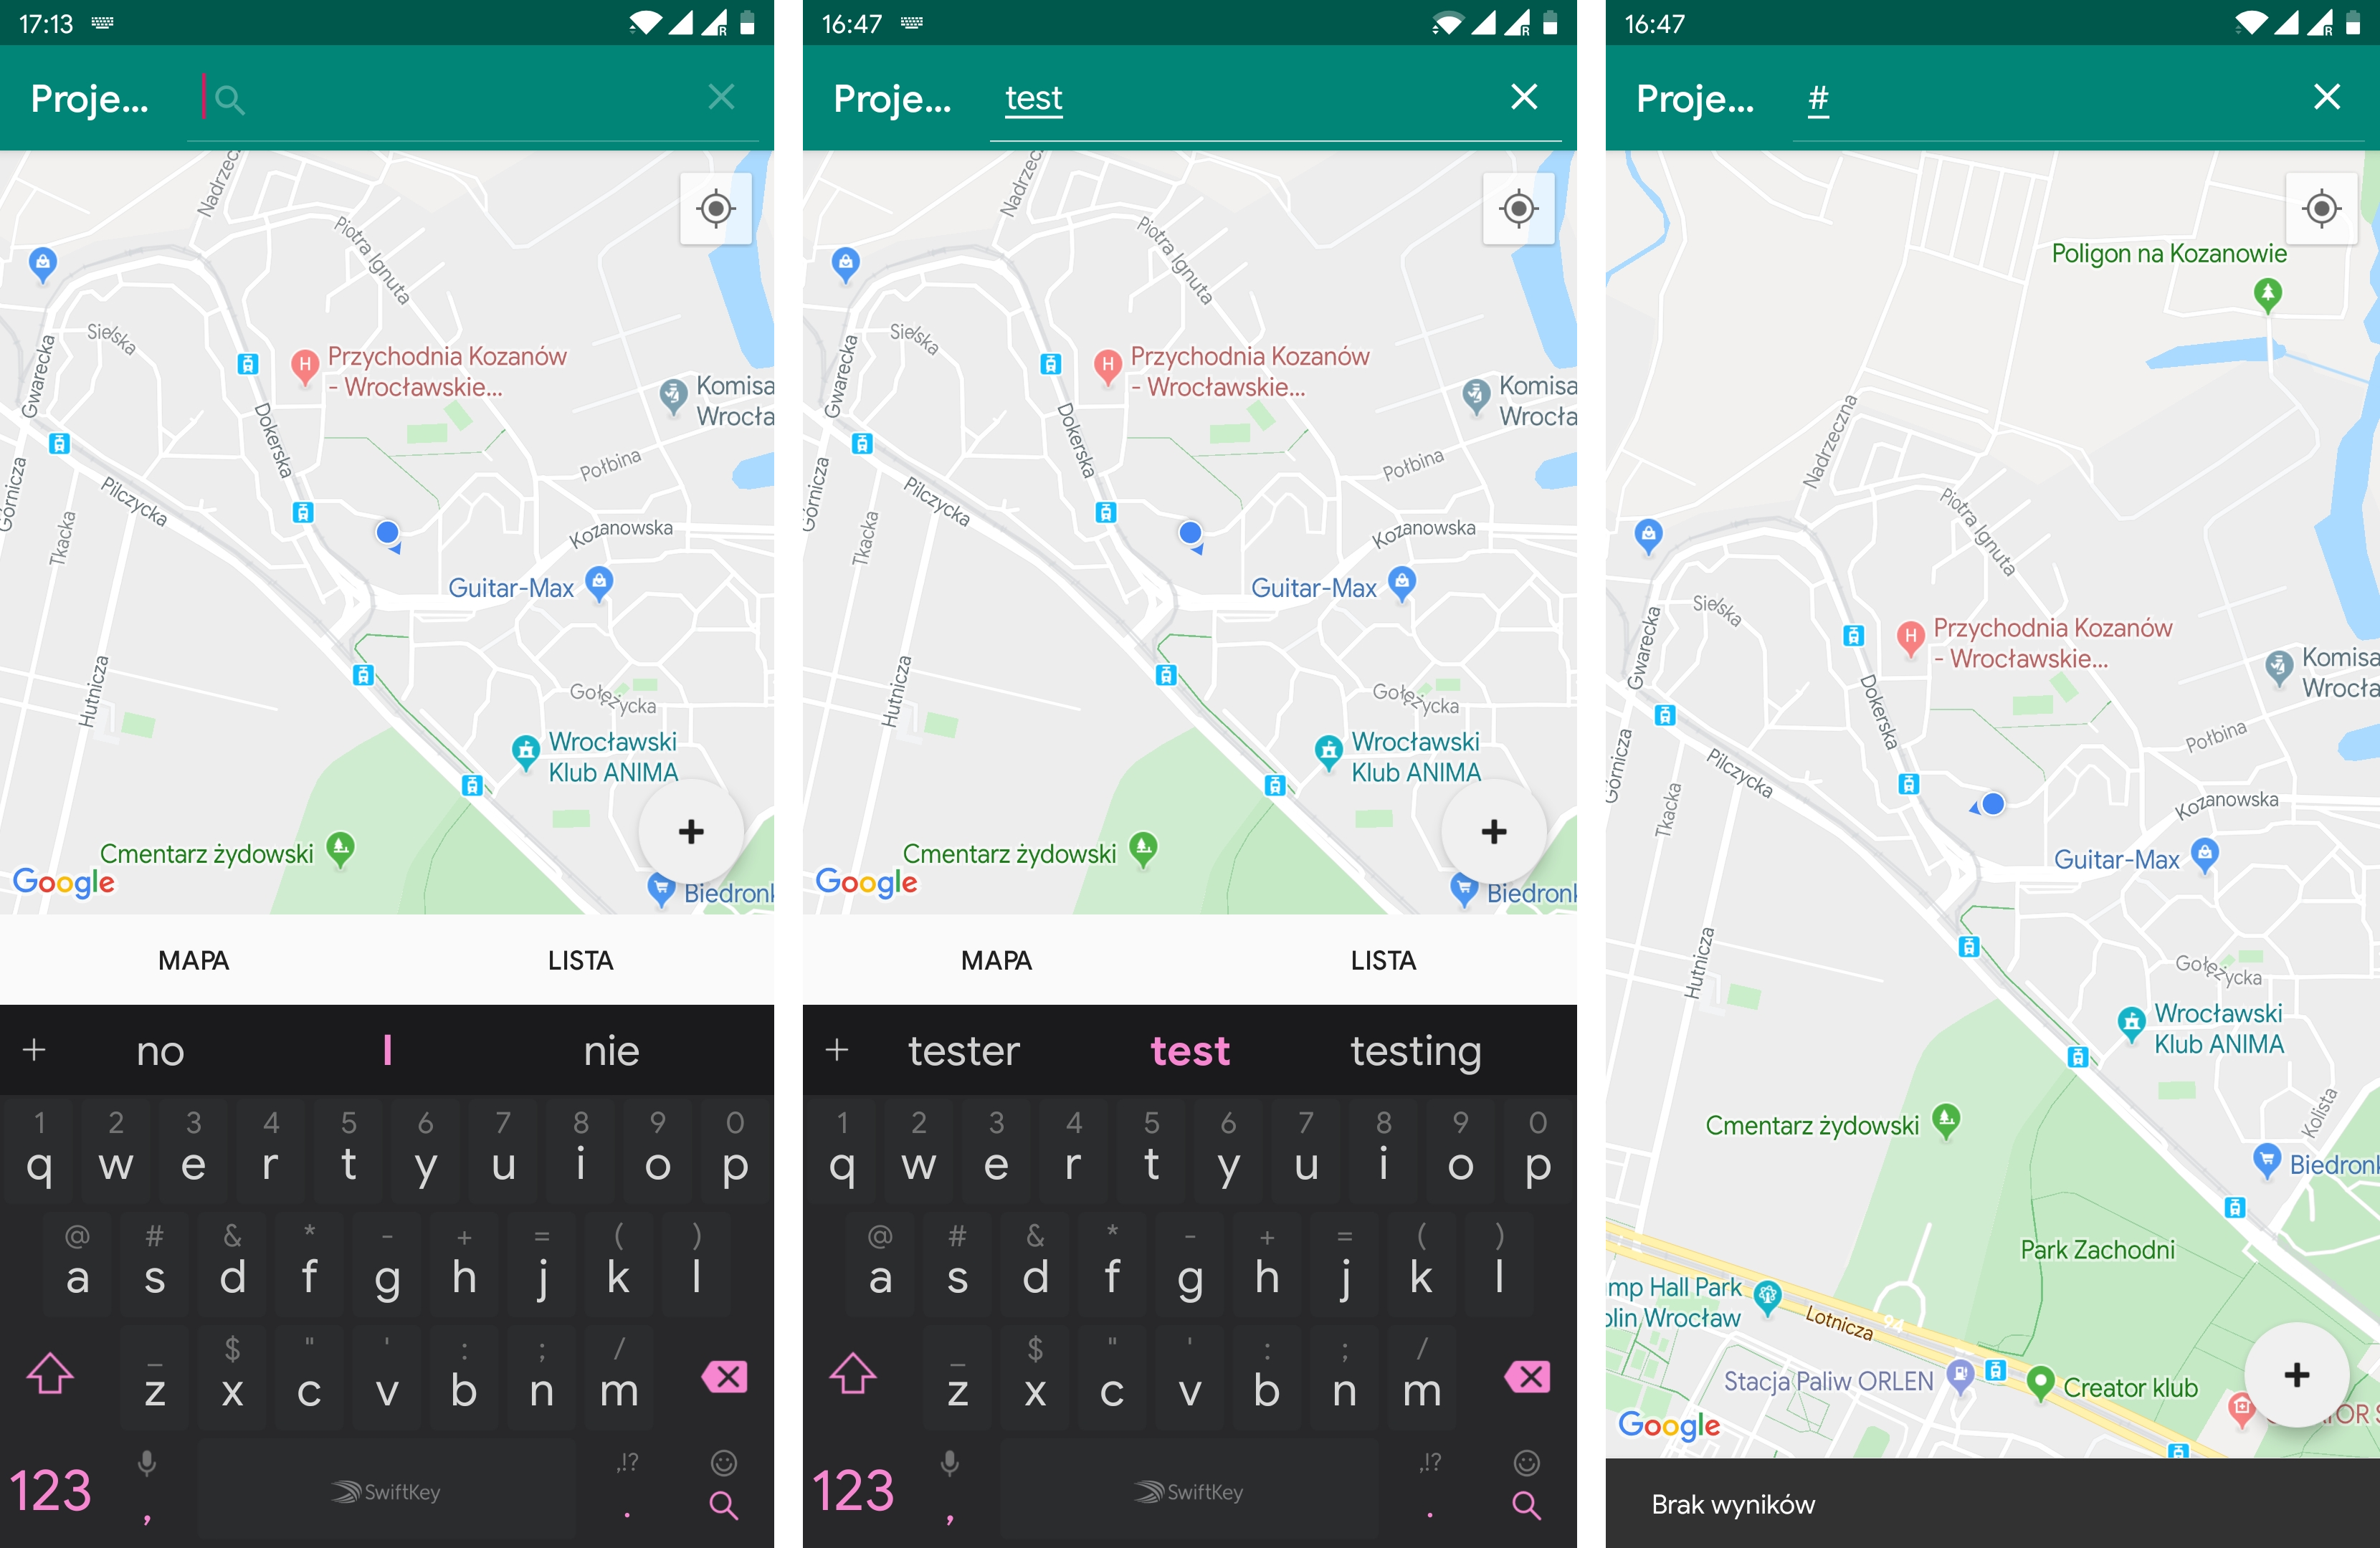
\includegraphics[width = \textwidth]{screenshot-search}
		\caption{Wygląd trybu wyszukiwania miejsc}
		\label{fig:screenshotsearch}
	\end{figure}

	Wyszukiwanie markerów na mapie odbywa się w widoku mapy. Po kliknięciu ikony wyszukiwania pojawia się pasek, gdzie należy wpisać szukany ciąg znaków. Miejsca przeszukiwane są po nazwie i adresie. Wyszukiwanie zatwierdzane jest za pomocą przycisku na klawiaturze ekranowej.

	W przypadku nieznalezienia żadnych wyników wyświetla się komunikat o błędzie, natomiast w przypadku powodzenia mapa ograniczy wyświetlane markery do tych spełniających kryteria wyszukiwania, a kamera przenosi się na pierwsze spełniające zapytanie miejsce.

	Opuszczenie wyszukiwania i powrót do wszystkich miejsc następuje poprzez kliknięcie przycisku X na pasku szukania.

	Ryc. \ref{fig:screenshotsearch} przedstawia po kolei: pasek wyszukiwania, pasek uzupełniony szukaną frazą oraz błąd, gdy nie znaleziono żadnych wyników.

	\subsection{Tryb edycji i dodawania obiektów}

	\begin{figure}[H]
		\centering
		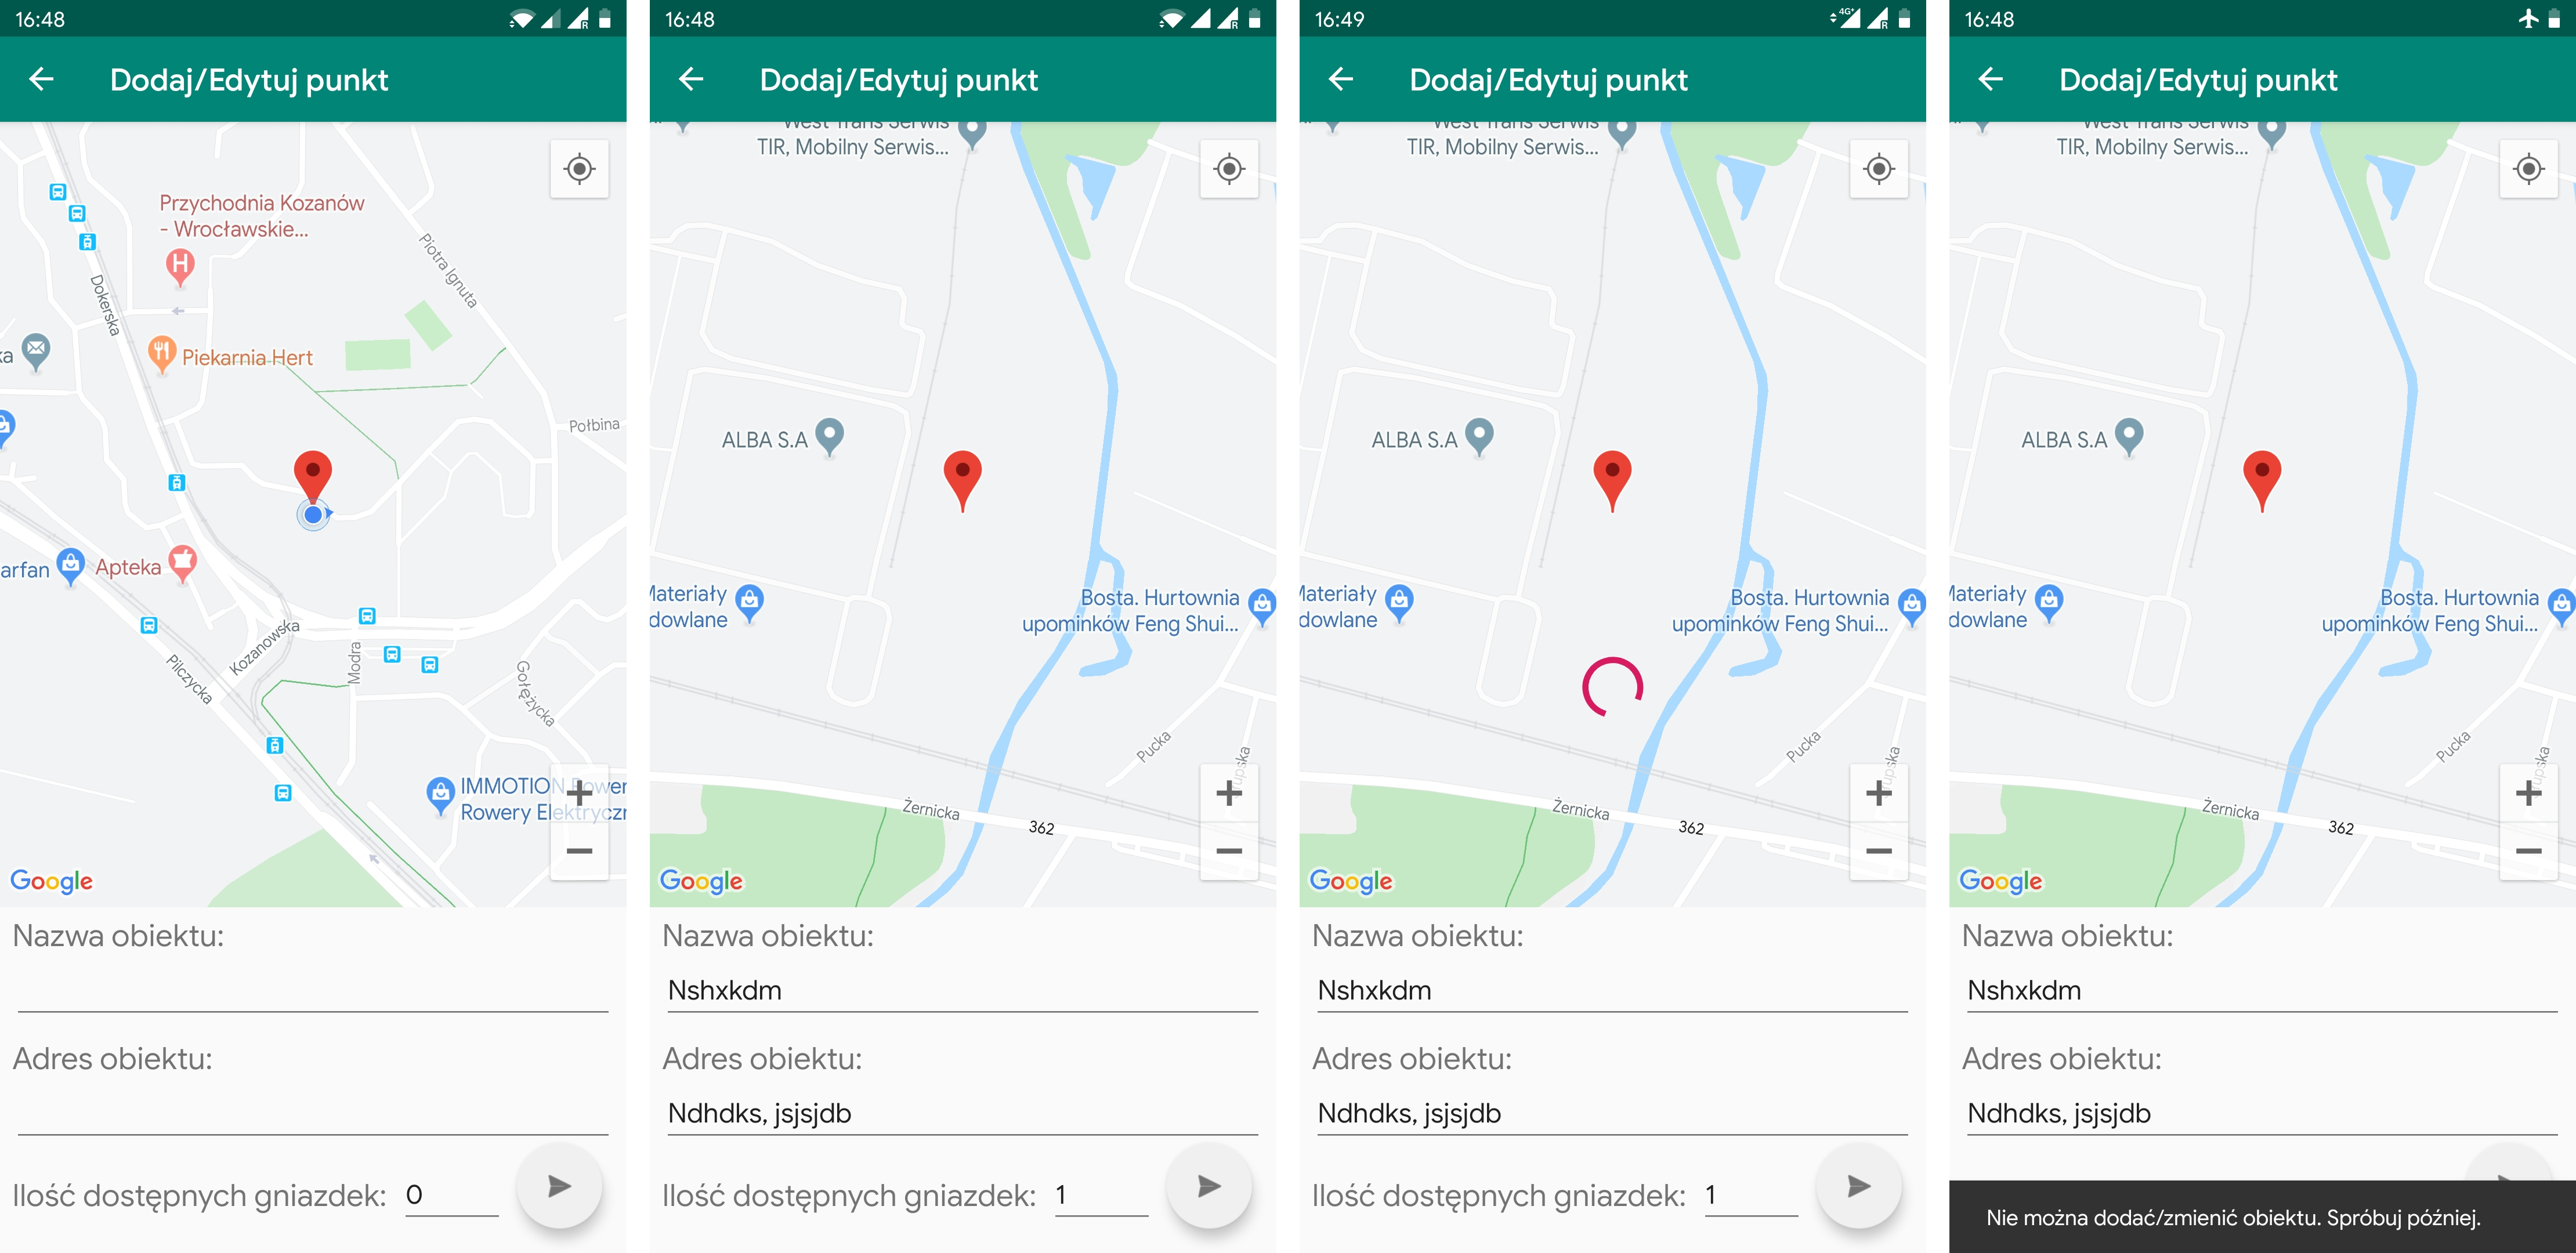
\includegraphics[width = \textwidth]{screenshot-addedit}
		\caption{Możliwy wygląd ekranu dodawania/edycji punktu na mapie}
		\label{fig:screenshotaddedit}
	\end{figure}

	Widok dodawania i edycji to jeden widok. W przypadku dodawania widok nie zawiera żadnych danych o miejscu, a marker na mapie wyświetla się na aktualnej lokalizacji użytkownika. W przypadku edycji widok wypełnia się aktualnym informacjami o miejscu.

	Zmiana pozycji markera odbywa się poprzez kliknięcie w nową lokalizację na mapie.

	Zapisanie danych jest możliwe po kliknięciu przycisku w prawym dolnym rogu. Przy zapisywaniu danych pojawia się nieskończony pasek postępu, który znika po zakończeniu procesu dodawania. Przy niepowodzeniu następuje wyświetlenie stosownego komunikatu, natomiast po poprawnym dodaniu aplikacja wraca do głównego ekranu mapy.

	Wyjście z ekranu bez zapisywania zmian jest możliwe, używając sprzętowego klawisza "cofnij" lub przycisku na górnej belce widoku.

	Ryc. \ref{fig:screenshotaddedit} przedstawia po kolei: widok po otwarciu trybu dodawania, widok trybu edycji, pasek postępu przy zapisywaniu zmian oraz komunikat o błędzie przy zapisywaniu.

	\subsection{Widok szczegółowy i usuwanie miejsc}

	\begin{figure}[H]
		\centering
		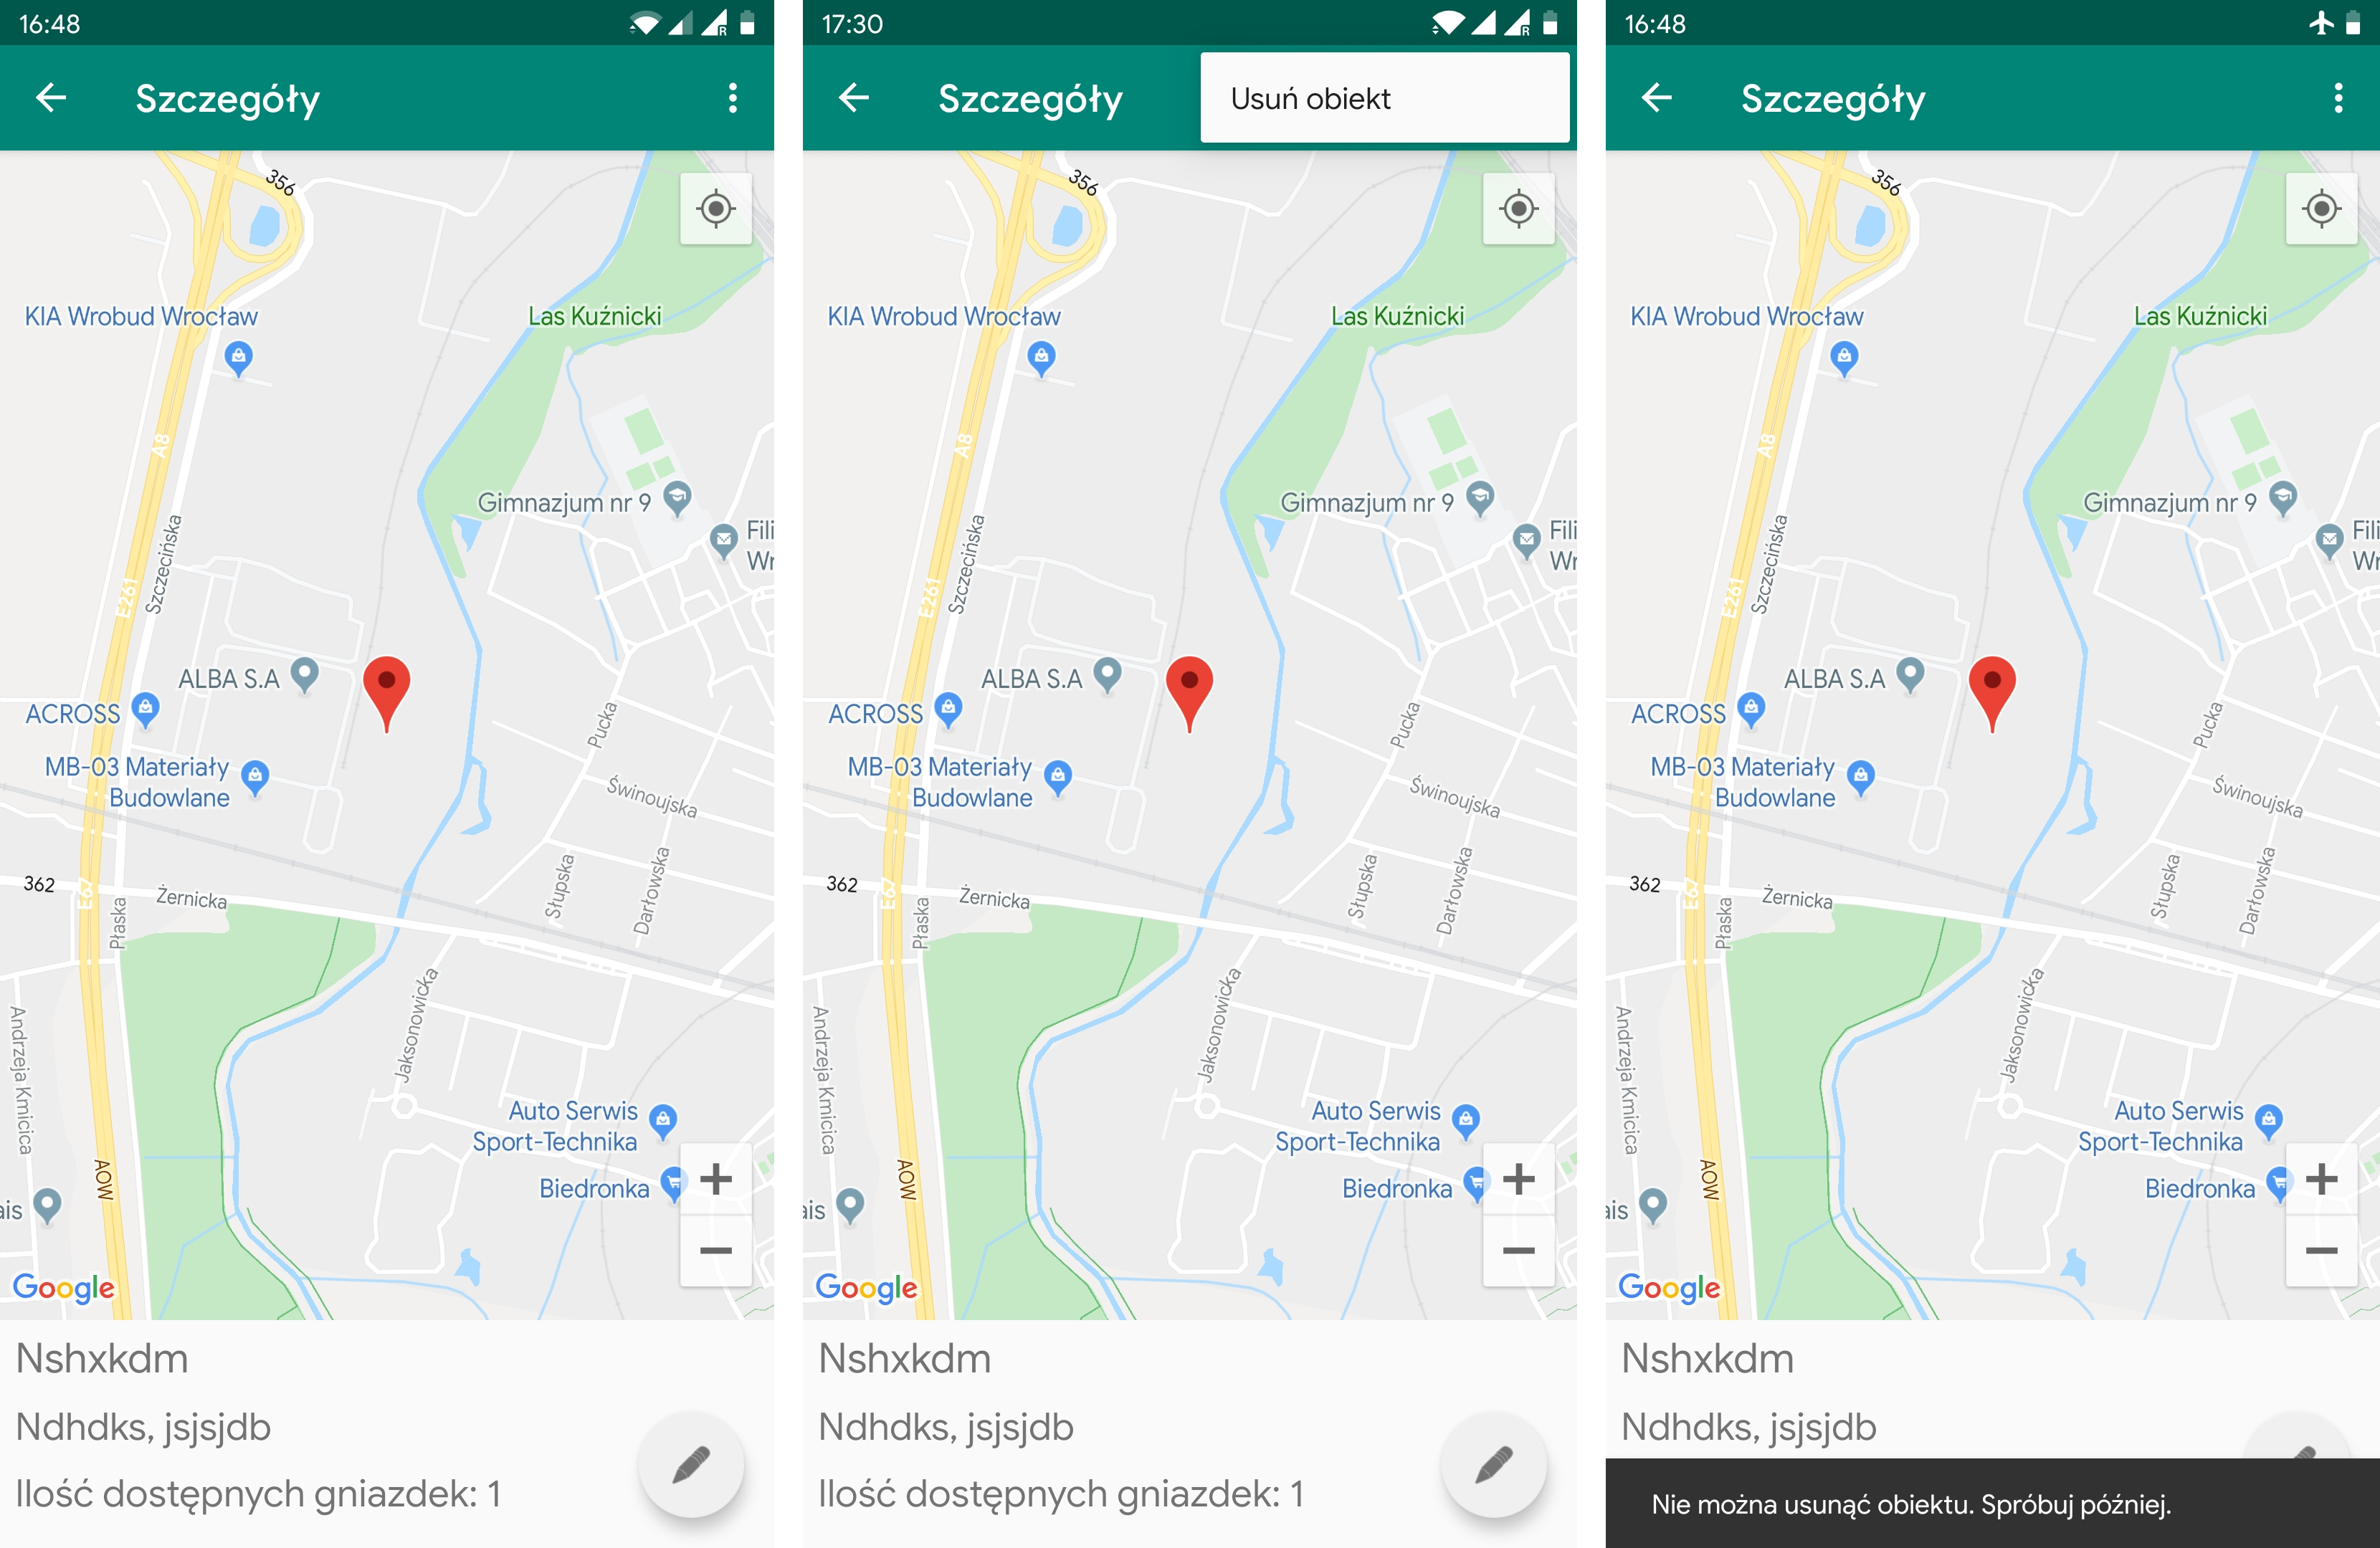
\includegraphics[width = \textwidth]{screenshot-detail}
		\caption{Ekran szczegółów wraz z błędem usuwania}
		\label{fig:screenshotdetail}
	\end{figure}

	Fragment ze szczegółami niewiele różni się wyglądem od trybu edycji. Nie oferuje on jednak możliwości zmiany żadnych informacji.

	Usunięcie miejsca jest możliwe z poziomu pozycji w menu na górnym pasku aplikacji. Po wywołaniu usuwania miejsca, tak jak w przypadku dodawania wyświetla się okrągły pasek postępu. Niepowodzenie jest sygnalizowane odpowiednim komunikatem, a sukces przejściem do głównego ekranu mapy.

	Z tego widoku możliwe jest również przejście do widoku edycji, korzystając z przycisku w prawym dolnym rogu. Wyjście, czyli powrót do widoku mapy lub listy jest możliwe używając sprzętowego przycisku, bądź przycisku na górnym pasku.

	Ryc. \ref{fig:screenshotdetail} przedstawia po kolei: widok szczegółów, menu widoku szczegółowego oraz błąd przy usuwaniu miejsca.

\section{Podsumowanie}\label{summary}

W ramach pracy dyplomowej zostały zaimplementowane podstawowe funkcjonalności opisane w koncepcie aplikacji, umożliwiające korzystanie z niej w założonych celach. Korzystając z programu da się oczywiście odczuć, że to nie jest jeszcze finalna wersja, jednak podstawowy zasób funkcji jest już dostępny. W dokumencie opisano metody realizacji każdej z tej funkcjonalności, na poziomie koncepcyjnym, jak i bardziej szczegółowym poziomie kodu.

Duża część czasu tworzenia tej pracy została poświęcona na zapoznanie się z językiem Kotlin oraz \texttt{Android Framework}. Podchodząc do realizacji pracy autor nie miał żadnego doświadczenia w obu tych dziedzinach, więc potrzebna była nauka od zera. Wykonanie tej pracy dało jej autorowi solidny zasób podstawowej znajomości tych technologii oraz poszerzyło jego umiejętności w programowaniu ogółem.

Aplikacja została zaprojektowana tak by wykorzystać jak najwięcej gotowych bibliotek wchodzących w skład frameworku Androida, ponieważ naturalnie domyślna implementacja dla danej platformy jest z reguły najbardziej optymalna do ogólnych zastosowań. W projekcie wykorzystano również dwie zewnętrzne biblioteki — Timber i Moshi. Wykorzystanie biblioteki Timber było spowodowane chęcią zachowania bardziej przejrzystego kodu. Zakres, w którym została ona wykorzystana pozwolił na bardziej czytelny kod odpowiedzialny za korzystanie z logów systemowych. Biblioteka Moshi natomiast zaoszczędziła autorowi pracy sporo czasu wymaganego na ręczną implementacje metod konwersji \texttt{JSON} na reprezentacje modelu danych i odwrotnie. Wykorzystanie zewnętrznej biblioteki gwarantuje, że dana funkcjonalność będzie poprawnie zaimplementowana i pozwala na skupienie się na implementacji funkcjonalności na wyższym poziomie. Dodatkowo zewnętrzna biblioteka została przez wiele osób już przetestowana i sprawdzona.

Dalszy rozwój projektu powinien skupić się na implementacji kolejnych funkcjonalności opisanych w rozdziale \ref{concept}, głównie na implementacji obsługi kont użytkownika oraz poprawieniu dość ascetycznego interfejsu użytkownika. Warto by również przeanalizować, jakie dokładnie dane powinny być przechowywane na temat poszczególnych punktów na mapie oraz poszerzona powinna zostać integracja z usługą \textit{Google Maps Services}. Rozwój tej aplikacji wymaga oczywiście pewnej dozy współpracy na poziomie planowania pomiędzy osobami odpowiedzialnymi za rozwój klienta oraz serwera internetowego.

\printbibliography[heading=bibintoc,title={Literatura}]

\renewcommand{\section}{\sectioncmd}
\clearpage

\listoffigures
\addcontentsline{toc}{section}{Indeks rycin}

\listoflistings
\addcontentsline{toc}{section}{Indeks listingów}

\end{document}
